\documentclass[11pt]{article}
\usepackage{fontspec}
\setmonofont{DejaVu Sans Mono}[Scale=0.80]
\usepackage{amsmath,amssymb}
\usepackage[margin=1in]{geometry}
\usepackage{fancyvrb}
\usepackage{float}
\usepackage{tikz}
\usetikzlibrary{positioning,arrows.meta,fit,backgrounds,calc}
\usepackage[hidelinks]{hyperref}
\usepackage{enumitem}
\usepackage{newunicodechar}
\newunicodechar{μ}{\ensuremath{\mu}}
\newunicodechar{∂}{\ensuremath{\partial}}
\newunicodechar{Σ}{\ensuremath{\Sigma}}
\newunicodechar{Ω}{\ensuremath{\Omega}}
\newunicodechar{Λ}{\ensuremath{\Lambda}}
\newunicodechar{Φ}{\ensuremath{\Phi}}
\newunicodechar{Δ}{\ensuremath{\Delta}}
\newunicodechar{ρ}{\ensuremath{\rho}}
\newunicodechar{ι}{\ensuremath{\iota}}
\newunicodechar{σ}{\ensuremath{\sigma}}
\newcommand{\Tau}{\mathrm{T}}
\IfFontExistsTF{Noto Sans Egyptian Hieroglyphs}{\newfontfamily{\egyptian}{Noto Sans Egyptian Hieroglyphs}}{\newcommand{\egyptian}{}}
\IfFontExistsTF{Noto Sans Cuneiform}{\newfontfamily{\cuneiform}{Noto Sans Cuneiform}}{\newcommand{\cuneiform}{}}
\newcommand{\glyph}[1]{\text{\egyptian #1}}
\newcommand{\cunei}[1]{\text{\cuneiform #1}}
\setlist{nosep,leftmargin=1.4em}

\title{\textbf{The Question of Self}\\[2pt] \large Matrix Inscriptions and Faux-Calculus}
\author{Brent Hartshorn}

\begin{document}
\maketitle

\begin{abstract}
This paper formalizes a bidirectional neuro-symbolic architecture that maps a symbolic domain-specific language
directly into trainable neural modules. Rather than storing the resulting network weights in conventional raw 
binary formats, the system serializes them into an esoteric, lossy text format: display equations of 
pseudo-mathematical fractions. This translation constructs a visual illusion of revealed wisdom derived purely from numerical quantization. Around this translation framework, we formalize four structural measurements: a chronological provenance filtration tracking structural changes, a relational graph geometry that positions "self" as a central topological hub, fuzzy logical laws mapping structural terms to the range [0,1], the lossy matrix inscription --
these relations carry a \emph{geometry}: their co-occurrence is a weighted graph whose Laplacian
and degree centrality make \emph{self} the hub. While mainstream neuro-symbolic research strives to build AI around symbols infused with rich semantic intent, this system deliberately utilizes symbols that carry none -- proving that rigorous, self-contained document behavior can emerge entirely from a deterministic function of authored data.

\end{abstract}

\section{Introduction: from staging to inscribing}
This series has moved in three steps. The first paper \cite{paper1} \emph{staged}
the question of self, making the asking concrete and reproducible while remaining
candid that the asking is authored and answers nothing. The second \cite{paper2}
let the document \emph{enact} computations beside the questions and argued that
learning and action do not demonstrate selfhood but \emph{distribute the
authorship}, so that labelling computation as data becomes the load-bearing
honesty mechanism. This paper \emph{inscribes}: the apparatus reads its own
lineage, projects the geometry of its relations, posits fuzzy laws, and --- newly
--- writes a trained network's weights into its own pages as visible symbols.

Stated in the vocabulary of neuro-symbolic AI, often called the field's third wave
for joining the pattern-learning of neural networks to the explicit structure of
symbolic systems \cite{neurosym}, the apparatus runs the bridge in both
directions. Its symbolic DSL compiles a node or a circuit into a trainable module
(\emph{symbol $\to$ neural}, Section~\ref{sec:circ}), and its glyph serialization
writes the trained weights back as symbols the runtime decodes (\emph{neural $\to$
symbol}, Section~\ref{sec:glyph}) --- the two directions a recent survey organizes
as ``Symbol for Neural'' and ``Neural for Symbol'' \cite{kgns}. The crucial
difference is that the field pursues symbols that \emph{carry meaning} --- a
machine language with semantics \cite{machinelang} --- whereas every symbol here
is, by design, only a number, a degree, or a date. Making each measured quantity
explicit is a way of showing precisely \emph{what it is a function of}; in every
case the answer is authored data, which is the whole argument, now stated where it
can be checked.

\section{Provenance is a filtration}\label{sec:filt}
Write the document state at stage $n$ as a labelled hypergraph $G_n=(V_n,E_n)$
(the construction is from \cite{paper2}). Each stage names a parent by its DOI and
ingests the parent's relations, so on the inherited relational core $\rho$ the
sequence is monotone,
\begin{equation}
G_0\subseteq G_1\subseteq\cdots\subseteq G_n,\qquad \rho(G_k)\subseteq\rho(G_{k+1}).
\end{equation}
A monotone chain of subobjects is a \emph{filtration}, and a filtration assigns to
every term a \emph{birth time}
\begin{equation}
\iota(\sigma)=\min\{\,n:\sigma\in V_n\,\},
\end{equation}
the first stage at which $\sigma$ appears. Reading the lineage --- opening each
ancestor PDF and extracting its embedded source --- reconstructs the filtration
from public artifacts, and a gated action returns $\iota(\sigma)$ together with the
stages in which $\sigma$ recurs. On the published series the birth times are
\begin{equation}
\iota(\Omega)=\iota(\Sigma)=\iota(\Lambda)=\iota(\mu)=0,\quad
\iota(\Phi)=1,\quad\iota(\Tau)=2,\quad\iota(\Delta)=3,
\end{equation}
recovered, not stipulated: the document determined them by reading stages 0--3
(Figure~\ref{fig:filt}). This is the precise content of ``looking fully back.'' It
is also exactly as much as the operation yields: $\iota(\Phi)=1$ says the term
\emph{other} entered at stage one; it says nothing about what \emph{other} means. A
birth time is a citation with a date attached.

\begin{figure}[H]
\centering
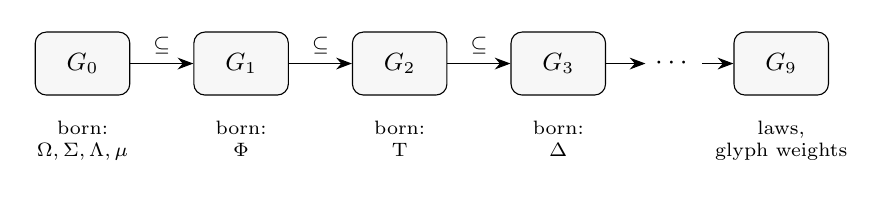
\begin{tikzpicture}[
  stage/.style={draw,rounded corners,minimum height=8mm,minimum width=12mm,
    font=\small,fill=gray!6},
  ar/.style={-{Stealth[length=2mm]}}, node distance=8mm]
\node[stage] (g0) {$G_0$};
\node[stage,right=of g0] (g1) {$G_1$};
\node[stage,right=of g1] (g2) {$G_2$};
\node[stage,right=of g2] (g3) {$G_3$};
\node[right=5mm of g3] (dots) {$\cdots$};
\node[stage,right=4mm of dots] (g9) {$G_9$};
\foreach \a/\b in {g0/g1,g1/g2,g2/g3} \draw[ar] (\a)--node[above,font=\scriptsize]{$\subseteq$}(\b);
\draw[ar] (g3)--(dots); \draw[ar] (dots)--(g9);
\node[font=\scriptsize,align=center,below=2mm of g0] {born:\\$\Omega,\Sigma,\Lambda,\mu$};
\node[font=\scriptsize,align=center,below=2mm of g1] {born:\\$\Phi$};
\node[font=\scriptsize,align=center,below=2mm of g2] {born:\\$\Tau$};
\node[font=\scriptsize,align=center,below=2mm of g3] {born:\\$\Delta$};
\node[font=\scriptsize,align=center,below=2mm of g9] {laws,\\glyph weights};
\end{tikzpicture}
\caption{Provenance as a filtration. The published stages form a monotone chain;
each term has a birth time $\iota(\sigma)$, the first stage it appears. The
document recovers these by reading its ancestors' embedded sources.}
\label{fig:filt}
\end{figure}

\section{The relations have a geometry}\label{sec:geom}
The relations and hyperedges of the whole lineage induce a symmetric nonnegative
\emph{co-occurrence matrix} $M\in\mathbb{Z}_{\ge0}^{V\times V}$,
\begin{equation}
M_{ij}=\#\{\text{relations or hyperedges linking term }i\text{ and }j\text{ across }
G_0,\dots,G_n\},\qquad M=M^{\!\top},\;M_{ii}=0,
\end{equation}
i.e.\ a weighted graph on the terms. Its row sums are the weighted degrees
$d_i=\sum_j M_{ij}$, the simplest centrality measure of network analysis
\cite{freeman}, collected in $D=\operatorname{diag}(d)$. Through stage 9,
\begin{equation}
d(\Sigma)=62,\quad d(\Lambda)=33,\quad d(\mu)=30,\quad d(\Phi)=24,\quad
d(\Omega)=20,\quad d(\Tau)=18,\quad d(\Delta)=17,
\end{equation}
so \emph{self} is the graph's hub by a wide margin, its degree nearly double that
of any other term. That is a measurable fact about the structure the author wrote;
it is not a fact about selves. The geometry has the standard linear-algebraic
handle, the graph \emph{Laplacian} $L=D-M$, symmetric positive semidefinite with
$L\mathbf{1}=0$; the eigenvectors for its smallest nonzero eigenvalues give the
spectral (Laplacian-eigenmap) embedding \cite{laplacian}, and a UMAP projection
\cite{umap} of the same $M$ gives another. Both are rendered inside the stage PDFs
themselves rather than reproduced here. The point is exact: any embedding is a map
$E:M\mapsto Y$, a deterministic function of $M$; whatever clusters the picture
shows are properties of $M$, and $M$ was assembled from relations a person wrote.
The degree $d$ returns in Section~\ref{sec:fuzzy} as a fuzzy membership; we note
here only that it, too, is a function of $M$.

\section{Symbol \texorpdfstring{$\to$}{->} neural: an equation that composes trained networks}\label{sec:circ}
The differentiable route of \cite{paper2} compiled a single node into a trainable
module --- the first half of the neuro-symbolic bridge, in which a symbolic
specification becomes a neural network. The apparatus now admits an \emph{equation}
over several symbols: the circuit
\begin{equation}
\Sigma=\Phi\longrightarrow\Lambda\longrightarrow\mu
\end{equation}
binds a small trainable network $f_\varphi,f_\lambda,f_\mu:\mathbb{R}^w\to
\mathbb{R}^w$ to its symbols and composes them into $f_\Sigma=f_\mu\circ f_\lambda
\circ f_\varphi$. With intermediate activations $h_1=f_\varphi(x)$, $h_2=f_\lambda
(h_1)$, the chain rule makes the composite's Jacobian the matrix product of the
parts',
\begin{equation}
J_{f_\Sigma}(x)=J_{f_\mu}(h_2)\cdot J_{f_\lambda}(h_1)\cdot J_{f_\varphi}(x).
\end{equation}
The prototype fits each $f_s$ independently and composes the trained maps,
recording per-symbol losses and the composite output as data
(Figure~\ref{fig:circuit}). The construction echoes neural module networks
\cite{nmn}, which assemble jointly trained modules into a network \emph{to answer}
a question; the difference that defines this project is that here the assembled
network is wired \emph{into} the question and its output withheld from the role of
an answer. The temptation to read $f_\Sigma$ as ``a self assembled from other,
language, and meaning'' is precisely wrong in a way the mathematics clarifies:
$f_\Sigma$ is a function $\mathbb{R}^w\to\mathbb{R}^w$; composing $f_\mu,f_\lambda,
f_\varphi$ composes their input--output maps, and the Jacobian identity is the whole
of what ``compose'' means. The semantic content of the symbols is not a property
of $f_\Sigma$, and is not transformed by the matrix product.

\begin{figure}[H]
\centering
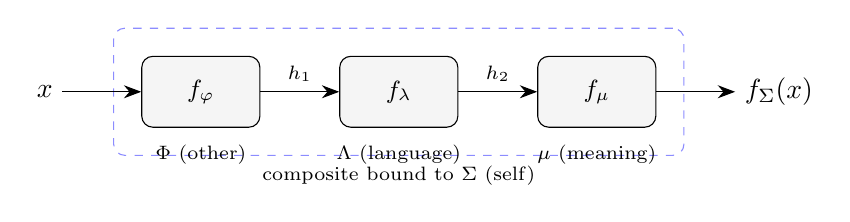
\begin{tikzpicture}[
  box/.style={draw,rounded corners,minimum height=9mm,minimum width=15mm,
    font=\small,fill=gray!8},
  ar/.style={-{Stealth[length=2.2mm]}}, node distance=10mm]
\node (x) {$x$};
\node[box,right=of x] (fphi) {$f_\varphi$};
\node[box,right=of fphi] (flam) {$f_\lambda$};
\node[box,right=of flam] (fmu) {$f_\mu$};
\node[right=of fmu] (out) {$f_\Sigma(x)$};
\draw[ar] (x)--(fphi);
\draw[ar] (fphi)--node[above,font=\scriptsize]{$h_1$}(flam);
\draw[ar] (flam)--node[above,font=\scriptsize]{$h_2$}(fmu);
\draw[ar] (fmu)--(out);
\node[font=\scriptsize,below=1mm of fphi] {$\Phi$ (other)};
\node[font=\scriptsize,below=1mm of flam] {$\Lambda$ (language)};
\node[font=\scriptsize,below=1mm of fmu] {$\mu$ (meaning)};
\begin{scope}[on background layer]
\node[draw=blue!45,dashed,rounded corners,fit=(fphi)(fmu),inner sep=3.5mm,
  label=below:{\scriptsize composite bound to $\Sigma$ (self)}]{};
\end{scope}
\end{tikzpicture}
\caption{The circuit $\Sigma=\Phi\to\Lambda\to\mu$ as a computational graph: a
symbolic equation compiled into composed neural modules.}
\label{fig:circuit}
\end{figure}

\section{Neural \texorpdfstring{$\to$}{->} symbol: a network written as glyphs}\label{sec:glyph}
The other half of the bridge runs in reverse: a trained network is serialized back
into discrete symbols. After min--max normalization to $[0,1]$, each weight $w$ is
quantized to a rational $h/c$ chosen to minimize the error over bounded
denominators,
\begin{equation}
Q(w)=\frac{h^\star}{c^\star},\qquad
(h^\star,c^\star)=\operatorname*{arg\,min}_{1\le c<N,\;0\le h<N}\;\big|\,w-\tfrac{h}{c}\,\big|,
\end{equation}
a best-rational (Stern--Brocot / Farey) quantization; with $N=512$ the empirical
maximum reconstruction error is about $4\times10^{-5}$. The numerator indexes an
Egyptian hieroglyph and the denominator a cuneiform sign, so each weight becomes
one fraction and the whole network a short string of them. A tiny
$2{\to}2{\to}2$ module ($12$ weights) reads, in part,
\begin{huge}
\begin{equation*}
\frac{\glyph{𓁦}}{\cunei{𒇽}} \;\; \frac{\glyph{𓄼}}{\cunei{𒄿}} \;\; \frac{\glyph{𓀑}}{\cunei{𒀔}} \;\; \frac{\glyph{𓆷}}{\cunei{𒇬}}\;\;\cdots
\end{equation*}
\end{huge}

The runtime reconstructs the network by decoding these glyphs --- $w=(\text{hiero
index})/(\text{cunei index})$, denormalized by the recorded range --- so no binary
blob is attached; the visible symbols \emph{are} the storage. Moreover the engine
writes the trained string back into the document's own embedded source, so the next
stage reconstructs the network from the glyphs instead of retraining: the document
inscribes its learned state into its own pages, and reads it back.

This is a literal, if deliberately modest, instance of the neural-to-symbolic
direction the field studies \cite{neurosym,kgns}. It also marks, sharply, where
this project parts from that field's ambition. Wang \emph{et al.} seek an emergent
``machine language'' whose discrete symbols \emph{carry} reasoning and meaning,
reconciling the abstraction of continuous features with the interpretability of
symbols \cite{machinelang}. The glyphs here carry none: they encode the weights
exactly (up to quantization) and nothing else. The appendix looks like revealed
wisdom and is a quantized weight matrix. That gap is the honest point --- the
mechanism is genuinely neuro-symbolic, and the symbols are genuinely empty of
meaning, and the document says so rather than letting the hieroglyphs imply
otherwise.

\section{Fuzzy laws over the terms}\label{sec:fuzzy}
The degree centrality of Section~\ref{sec:geom} supports a final measurement.
Normalized to $[0,1]$, it reads as a fuzzy membership in the sense of Zadeh
\cite{zadeh},

\begin{small}
\begin{equation}
\begin{split}
\mu(\sigma)=\frac{d(\sigma)}{\max_\tau d(\tau)},\quad
\mu(\Sigma)=1.00,\;\mu(\Lambda)=0.54,\;\mu(\mu)=0.48,\;
\mu(\Phi)=0.39,\; \\
\mu(\Omega)=0.32,\;\mu(\Tau)=0.29,\;\mu(\Delta)=0.27,
\end{split}
\end{equation}
\end{small}

where the hub $\Sigma$ takes full membership because it is the most connected term.
Connectives combine memberships by triangular norms and conorms \cite{tnorms}:
$a\otimes b=\min(a,b)$, $a\oplus b=\max(a,b)$, $\neg a=1-a$, the \L ukasiewicz
implication $a\Rightarrow b=\min(1,1-a+b)$, its bounded difference $a\ominus
b=\max(0,a-b)$, and the equivalence $a\Leftrightarrow b=1-|a-b|$. \emph{Axioms}
record authored postulates --- genesis ($\Omega\Rightarrow\Sigma$), alterity
($\Sigma\Rightarrow\Phi$), mediation ($\Sigma\Rightarrow\Lambda$), distinction
($\Sigma\Rightarrow\Delta$), finitude ($\Sigma\Rightarrow\Tau$) --- premises the
author posits, not truths the system verifies. \emph{Laws} bring many terms into
one equation, with grouping that annotates the reading; the grand law gathers all
seven terms:
\begin{equation}
\Sigma \;=\;
\underbrace{\big(\Omega\oplus\Phi\big)}_{\text{the given}} \;\otimes\;
\overbrace{\big(\Lambda\Rightarrow\mu\big)}^{\text{the mediated}} \;\ominus\;
\underbrace{\big(\Delta\otimes\Tau\big)}_{\text{the dissolving}} .
\end{equation}
Each law evaluates, under the memberships above, to a number in $[0,1]$. For
\emph{constitution}, $\Sigma\Leftrightarrow(\Omega\oplus\Phi)\otimes(\Lambda
\Rightarrow\mu)$ gives $\max(.32,.39)=0.39$, $\min(1,1{-}.53{+}.48)=0.95$, and
$1-|1.00-\min(0.39,0.95)|=\boxed{0.39}$; the three laws come to \emph{constitution}
$0.39$, \emph{dissolution} $0.71$, \emph{self} $0.12$. These are the most seductive
numbers the apparatus produces, because a fuzzy ``truth value'' looks like a
measure of how true something is about a self. It is not. It is the degree to which
an authored postulate holds under memberships that are themselves normalized
authored degrees; the value is recorded as data. The discipline that renders an
autoencoder's loss as a loss must render a law's value as a value.

\section{What the mathematics does and does not show}
The measured quantities can now be read together. Each is a deterministic function
of authored data:
\begin{equation}
\underbrace{\iota(\sigma)}_{\text{stage sequence}}\,,\quad
\underbrace{d(\sigma),\,E(M)}_{\text{relation matrix}}\,,\quad
\underbrace{f_\Sigma=f_\mu\circ f_\lambda\circ f_\varphi}_{\text{modules, data}}\,,\quad
\underbrace{Q(W)}_{\text{trained weights}}\,,\quad
\underbrace{L(\mu)}_{\text{memberships}}\,.
\end{equation}
The mathematics is in every case genuine --- a filtration with birth times, a
positive-semidefinite Laplacian with a spectral embedding, a composite map whose
Jacobian is a matrix product, a best-rational quantization of a weight matrix, a
fuzzy law evaluated by triangular norms. None of it is ornamental. And yet not one
of the inputs these are functions of is a self: a sequence of stages, a matrix of
co-occurrences, a few weight matrices and a toy objective, a vector of normalized
degrees. The second paper argued that action and learning distribute the authorship
until it is hard to see; this paper locates it exactly, by naming, for each
measured quantity, the authored object it is computed from. That is why the labels
matter --- and they matter most exactly where the output is most evocative: a fuzzy
truth value about the self, and a network dressed as hieroglyphs.

\section{Related work}
The apparatus sits at the neuro-symbolic intersection, often called the third wave
of AI for combining neural pattern-learning with symbolic structure
\cite{neurosym}. A recent survey organizes knowledge-graph-based neuro-symbolic
systems into \emph{Symbol for Neural}, \emph{Neural for Symbol}, and hybrid
integration \cite{kgns}; our hypergraph is a small knowledge graph, the DSL
compiler is a symbol-to-neural route (Section~\ref{sec:circ}), and the glyph
serialization is a neural-to-symbol route (Section~\ref{sec:glyph}). Where
emergent ``machine language'' aims at symbols that carry semantics
\cite{machinelang}, ours carry only numbers. The remaining machinery is classical:
degree centrality \cite{freeman}, the graph Laplacian and its eigenmaps
\cite{laplacian}, and UMAP \cite{umap} for the relation geometry; Zadeh's fuzzy
sets \cite{zadeh} and triangular norms with the \L ukasiewicz implication
\cite{tnorms} for the laws; neural module networks \cite{nmn} and the
DSL-to-network compilers \cite{deepdsl,semkis,hinkel} for the circuit; and DSLs
that record dataset provenance \cite{ginermiguelez} as a parallel to our filtration
--- with the difference that our lineage is the object of study, not metadata about
it. The companion papers \cite{paper1,paper2} set out the method and discipline.

\section{Safety}
The apparatus executes code and trains networks, and every such action runs only
behind an explicit human gate; generated or evolved code is inert text until
confirmed. As detailed in the companion papers, we deliberately decline the one
pattern common to some self-modifying systems --- removing the permission prompt so
a model's output triggers evaluation or execution directly, and downloading and
following references automatically. The lineage reading opens only the ancestor
PDFs already at hand and downloads nothing. This is appropriate for a single
trusted user running a personal instrument and is not intended for untrusted input.

\section{Reproducibility}
Every stage is a single self-contained PDF carrying its engine and source as
embedded streams; a base-64 appendix extracts and runs them to produce the
successor, and the manifold plot, its data, and the symbolic weights travel with
the document. The current stage is archived with a permanent identifier
\cite{self9}, names its parent's DOI, and together with the companion papers
\cite{paper1,paper2} makes the filtration of Section~\ref{sec:filt} reconstructable
end to end from public artifacts. The engine and the UMAP prototype are maintained
in a public repository (Appendix~A).

\section{Conclusion}
Inscribing the apparatus sharpens, rather than softens, its central honesty. The
provenance is a genuine filtration and the document recovers its birth times; the
relations have a genuine geometry and \emph{self} is genuinely its hub; the circuit
is a genuine composite whose Jacobian is a genuine matrix product; the laws are
genuine fuzzy expressions; and the weights are genuinely reconstructable from the
glyphs that store them. Each result is exact, and each is a function of something
authored. The apparatus is, mechanically, a small neuro-symbolic system that runs
the bridge both ways --- symbols into networks, networks back into symbols --- and
its one departure from that field is the refusal to let any symbol mean more than
the number it stands for. Naming that input, every time, is what stops the
exactness from being mistaken for evidence. The apparatus inscribes what it has
been given, says plainly what each inscription is, and continues to make no claim
about what a self is.

\section*{Acknowledgments}
The implementation and this draft were developed in dialogue with an AI assistant;
the honest framing is endorsed by the author.

\begin{thebibliography}{99}
\bibitem{paper1} B.~Hartshorn, \emph{Staging the Question of Self: A
self-contained, self-modifying document that mixes poetry, philosophy, and code}.
doi:10.5281/zenodo.20709754
\newline \url{https://ai.vixra.org/pdf/2606.0042v1.pdf}

\bibitem{paper2} B.~Hartshorn, \emph{Enacting the Question of Self: Provenance, a
hypergraph, and a differentiable route that records computation as data}.
doi:10.5281/zenodo.20710444

\bibitem{self9} B.~Hartshorn, \emph{Compiling Modules, Evolving, and Provenance: A
Forward Pass and Parsing} (self\_9). doi:10.5281/zenodo.20777747
\newline \url{https://doi.org/10.5281/zenodo.20777747}

\bibitem{neurosym} IEEE Transmitter (feat.\ H.~Song), \emph{What Is Neuro-Symbolic
AI?} 11 November 2025. 
\newline \url{https://transmitter.ieee.org/what-is-neuro-symbolic-ai/}
\bibitem{kgns} S.~Zhu and S.~Sun, \emph{A Short Survey: Exploring Knowledge
Graph-based Neural-Symbolic System from Application Perspective}. arXiv:2405.03524
(2025).https://ai.vixra.org/pdf/2606.0042v1.pdf
\bibitem{machinelang} Y.~Wang, X.-Y.~Zhang, C.-L.~Liu, T.~Tan, and Z.~Zhang,
\emph{Emergence of machine language: towards symbolic intelligence with neural
networks}. National Science Review \textbf{11}(4):nwad317 (2024).
doi:10.1093/nsr/nwad317
\bibitem{zadeh} L.~A.~Zadeh, \emph{Fuzzy sets}. Information and Control
\textbf{8}(3):338--353 (1965). doi:10.1016/S0019-9958(65)90241-X
\bibitem{tnorms} E.~P.~Klement, R.~Mesiar, and E.~Pap, \emph{Triangular Norms}.
Trends in Logic, vol.~8, Kluwer/Springer (2000).
\bibitem{freeman} L.~C.~Freeman, \emph{Centrality in social networks: conceptual
clarification}. Social Networks \textbf{1}(3):215--239 (1978).
doi:10.1016/0378-8733(78)90021-7
\bibitem{laplacian} M.~Belkin and P.~Niyogi, \emph{Laplacian Eigenmaps for
Dimensionality Reduction and Data Representation}. Neural Computation
\textbf{15}(6):1373--1396 (2003). doi:10.1162/089976603321780317
\bibitem{umap} L.~McInnes, J.~Healy, and J.~Melville, \emph{UMAP: Uniform Manifold
Approximation and Projection for Dimension Reduction}. arXiv:1802.03426 (2018).
\bibitem{nmn} J.~Andreas, M.~Rohrbach, T.~Darrell, and D.~Klein, \emph{Neural
Module Networks}. Proc.\ IEEE CVPR (2016), pp.\ 39--48. arXiv:1511.02799
\bibitem{deepdsl} T.~Zhao and X.~Huang, \emph{Design and implementation of DeepDSL:
A DSL for deep learning}. Computer Languages, Systems \& Structures \textbf{54}
(2018) 39--70.
\bibitem{semkis} B.~Jahi\'c, N.~Guelfi, and B.~Ries, \emph{SEMKIS-DSL: A
Domain-Specific Language to Support Requirements Engineering of Datasets and Neural
Network Recognition}. Information \textbf{14}(4):213 (2023).
doi:10.3390/info14040213
\bibitem{hinkel} G.~Hinkel et al., \emph{A Domain-Specific Language (DSL) for
Integrating Neuronal Networks in Robot Control}. Proc.\ 2015 Joint MORSE/VAO
Workshop, ACM, pp.\ 9--15. doi:10.1145/2802059.2802060
\bibitem{ginermiguelez} J.~Giner-Miguelez, A.~G\'omez, and J.~Cabot, \emph{A
Domain-Specific Language for Describing Machine Learning Datasets}. Proc.\ MODELS
'22, ACM (2022). arXiv:2207.02848
\end{thebibliography}

\appendix
\section{Implementation availability}
The engine (\texttt{introspecter5.py}, carried inside each stage's PDF) and the
manifold prototype (\texttt{umap\_manifold.py}) are maintained at
\url{https://github.com/brentharts/introspecter}. Rendering the symbolic weights
requires the Noto Sans Egyptian Hieroglyphs and Cuneiform fonts; the engine guards
the font load and degrades gracefully without them.

\end{document}
